\documentclass{article}
\usepackage{tikz}
\usetikzlibrary{matrix,positioning,arrows.meta,shapes.arrows}
\begin{document}
Drawing Triangles

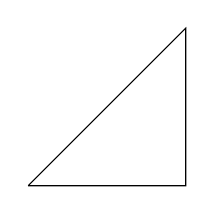
\begin{tikzpicture}
\draw (0,0) -- (2,2) -- (2,0) -- (0,0);
\end{tikzpicture}

Scaling pictures

\begin{tikzpicture}[scale=3]
\draw (0,0) -- (2,2) -- (2,0) -- (0,0);
\end{tikzpicture}

Line thickness. Options are: ultra thin, very thin, thin, semithick, thick,
very thick and ultra thick, as well as help lines

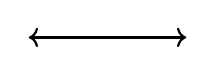
\begin{tikzpicture}
\draw[thick,<->] (0,0) -- (2,0);
\end{tikzpicture}

Drawing Circles

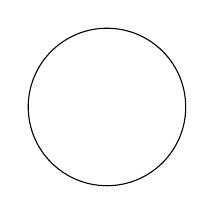
\begin{tikzpicture}
\draw (0,0) circle (1);
\end{tikzpicture}

Drawing Grids

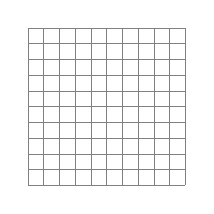
\begin{tikzpicture}
\draw[help lines,step=0.2cm] (-1,-1) grid (1,1);
\end{tikzpicture}

Drawing Parabola

\begin{tikzpicture}
% Draw the x and y axes first
\draw (-2,0) -- (2,0);
\draw (0,-2) -- (0,2);
% Need to figure out how to specify a third point to 
% make it a proper parabola
\draw (-2,-1) parabola (2,2);
\end{tikzpicture}

Drawing Arcs

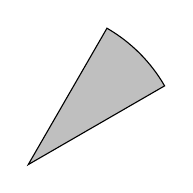
\begin{tikzpicture}
% The arc command has 3 arguments - start angle, end angle and circle radius
% The gray!50 means 50% gray
% I think the + before a coordinate makes it relative
\draw[fill=gray!50] (1,0) -- +(30:2) arc (30:60:2) -- cycle;
\end{tikzpicture}

Using relative arguments:

The + is maintained with respect to the first coordinate given, not just the
previous one. In this example, it will draw a line up, then horizontally to
the right, as opposed to a line up, then diagonally up
If you want to maintain relative coordinates with respect to the last point
placed, use ++
\begin{tikzpicture}
%\draw (1,0) -- (30:2); 
%\draw (1,0) -- +(30:2); 
\draw (0,0) -- +(0,1);  -- +(1,1);
\draw (0,-4) -- ++(0,1); -- ++(1,0);
\end{tikzpicture}

Adding text to images

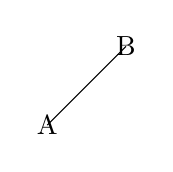
\begin{tikzpicture}
\draw (1,1) node{A} -- (2,2) node{B};
\end{tikzpicture}

Not very nice at first, can use the anchor option to make it better

\begin{tikzpicture}
\draw (1,1) node[anchor=north east]{A} -- (2,2) node[anchor=south west]{B};
\end{tikzpicture}

Can even add some circle bounding boxes

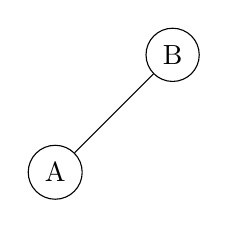
\begin{tikzpicture}
\draw (1,1) node[anchor=north east,circle,draw]{A} -- (2,2) node[anchor=south
west,circle,draw]{B};
\end{tikzpicture}

Simple labels can use the label option

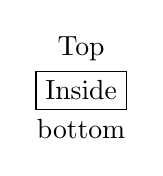
\begin{tikzpicture}
\draw (1,1) node[rectangle,draw,label=above:Top,label=below:bottom]{Inside}; 
\end{tikzpicture}

Or the pin option, if you want latex to draw a line to your node

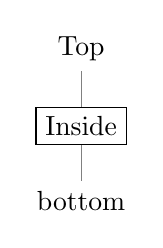
\begin{tikzpicture}
\draw (1,1) node[rectangle,draw,pin=above:Top,pin=below:bottom]{Inside}; 
\end{tikzpicture}

To draw things with a large number of coordinates, we can use the plot command.
The nice thing about this is you now specify the start and end coordinates. Use
\emph{-- --plot} to keep drawing when you go to the next start coordinate, or simply
\emph{plot} to lift the pen up and move it to the next coordinate.

With --plot:

\begin{tikzpicture}
\draw (0,0) -- (1,0) --plot coordinates {(2,-1) (2,1)};
\end{tikzpicture}

With standard plot:

\begin{tikzpicture}
\draw (0,0) -- (1,0) plot coordinates {(2,-1) (2,1)};
\end{tikzpicture}

And finally, we can draw complex functions, but this will require an external
call to gnuplot

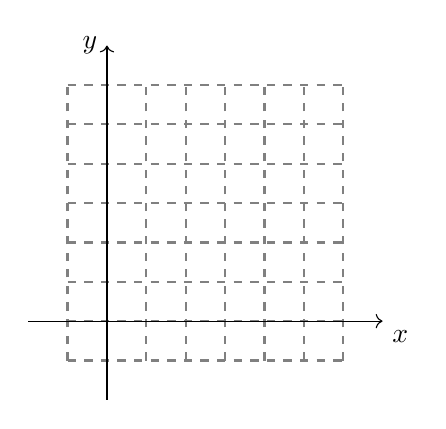
\begin{tikzpicture}[domain=0:2]
\draw[thick,color=gray,step=.5cm,dashed] (-0.5,-.5) grid (3,3);
\draw[->] (-1,0) -- (3.5,0) node[below right] {$x$};
\draw[->] (0,-1) -- (0,3.5) node[left] {$y$};
\draw plot[id=x] function{x*x};
\end{tikzpicture}

Tikz also allows you to plot functions without having to use external programs,
but the subset is limited (although should suffice for most things)

\begin{tikzpicture}[xscale=13,yscale=3.8]
\draw [<->] (0,0.8) -- (0,0) -- (0.5,0);
\draw[green, thick, domain=0:0.5] plot (\x, {0.025+\x+\x*\x});
\end{tikzpicture}

For example, here's a complex gabor wavelet

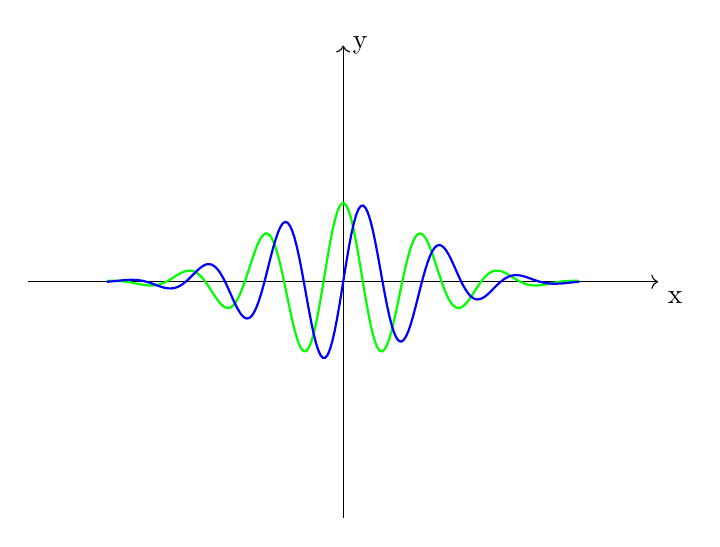
\begin{tikzpicture}
\draw[->] (-4,0) -- (4,0) node[below right] {x};
\draw[->] (0,-3) -- (0,3) node[right] {y};
\draw[green, thick, domain=-3:3, samples=200] plot (\x, {exp(-pow(\x,2)/2) * cos(2*pi*\x r)});
\draw[blue, thick, domain=-3:3, samples=200] plot (\x, {exp(-pow(\x,2)/2) * sin(2*pi*\x r)});
\end{tikzpicture}

What about something more advanced? Here's a neural network I got from the web

\def\layersep{2.5cm}

\begin{tikzpicture}[shorten >=1pt,->,draw=black!50, node distance=\layersep]
    \tikzstyle{every pin edge}=[<-,shorten <=1pt]
    \tikzstyle{neuron}=[circle,fill=black!25,minimum size=17pt,inner sep=0pt]
    \tikzstyle{input neuron}=[neuron, fill=green!50];
    \tikzstyle{output neuron}=[neuron, fill=red!50];
    \tikzstyle{hidden neuron}=[neuron, fill=blue!50];
    \tikzstyle{annot} = [text width=4em, text centered]

    % Draw the input layer nodes
    \foreach \name / \y in {1,...,4}
    % This is the same as writing \foreach \name / \y in {1/1,2/2,3/3,4/4}
        \node[input neuron, pin=left:Input \#\y] (I-\name) at (0,-\y) {};

    % Draw the hidden layer nodes
    \foreach \name / \y in {1,...,5}
        \path[yshift=0.5cm]
            node[hidden neuron] (H-\name) at (\layersep,-\y cm) {};

    % Draw the output layer node
    \node[output neuron,pin={[pin edge={->}]right:Output}, right of=H-3] (O) {};

    % Connect every node in the input layer with every node in the
    % hidden layer.
    \foreach \source in {1,...,4}
        \foreach \dest in {1,...,5}
            \path (I-\source) edge (H-\dest);

    % Connect every node in the hidden layer with the output layer
    \foreach \source in {1,...,5}
        \path (H-\source) edge (O);

    % Annotate the layers
    \node[annot,above of=H-1, node distance=1cm] (hl) {Hidden layer};
    \node[annot,left of=hl] {Input layer};
    \node[annot,right of=hl] {Output layer};
\end{tikzpicture}

And for a 3D network:

%transforms all coordinates the same way when used (use it within a scope!)
%(rotation is not 45 degress to avoid overlapping edges)
% Input: point of origins x and y coordinate
\newcommand{\myGlobalTransformation}[2] {%
    \pgftransformcm{1}{0}{0.4}{0.5}{\pgfpoint{#1cm}{#2cm}}
}

% draw a 4x4 helper grid in 3D
% Input: point of origins x and y coordinate and additional drawing-parameters
\newcommand{\gridThreeD}[3]{%
    \begin{scope}
        \myGlobalTransformation{#1}{#2};
        \draw [#3,step=2cm] grid (8,8);
    \end{scope}
}

\tikzstyle myBG=[line width=3pt,opacity=1.0]

% draws lines with white background to show which lines are closer to the
% viewer (Hint: draw from bottom up and from back to front)
%Input: start and end point
\newcommand{\drawLinewithBG}[2] {%
    \draw[white,myBG]  (#1) -- (#2);
    \draw[black,very thick] (#1) -- (#2);
}

% draws all horizontal graph lines within grid
\newcommand{\graphLinesHorizontal} {%
    \drawLinewithBG{1,1}{7,1};
    \drawLinewithBG{1,3}{7,3};
    \drawLinewithBG{1,5}{7,5};
    \drawLinewithBG{1,7}{7,7};
}

% draws all vertical graph lines within grid
\newcommand{\graphLinesVertical} {%
    %swaps x and y coordinate (hence vertical lines):
    \pgftransformcm{0}{1}{1}{0}{\pgfpoint{0cm}{0cm}}
    \graphLinesHorizontal;
}

%draws nodes of the grid
%Input: point of origins x and y coordinate
\newcommand{\graphThreeDnodes}[2] {%
    \begin{scope}
        \myGlobalTransformation{#1}{#2};
        \foreach \x in {1,3,5,7} {%
            \foreach \y in {1,3,5,7} {%
                \node at (\x,\y) [circle,fill=black] {};
                %this way circle of nodes will not be transformed
            }
        }
    \end{scope}
}


\begin{tikzpicture}

    %draws helper-grid:
    \gridThreeD{0}{0}{black!50};
    \gridThreeD{0}{4.25}{black!50};

    %draws lower graph lines and those in z-direction:
    \begin{scope}
        \myGlobalTransformation{0}{0};
        \graphLinesHorizontal;

        %draws all graph lines in z-direction (reset transformation first!):
        \foreach \x in {1,3,5,7} {%
            \foreach \y in {1,3,5,7} {%
                \node (thisNode) at (\x,\y) {};{%
                    \pgftransformreset
                    \draw[white,myBG]  (thisNode) -- ++(0,4.25);
                    \draw[black,very thick] (thisNode) -- ++(0,4.25);
                }
            }
        }
    \end{scope}

    %draws upper graph-lines:
    \begin{scope}
        \myGlobalTransformation{0}{4.25};
        \graphLinesVertical;
    \end{scope}

    % draws all graph nodes:
    \graphThreeDnodes{0}{0};
    \graphThreeDnodes{0}{4.25};

\end{tikzpicture}

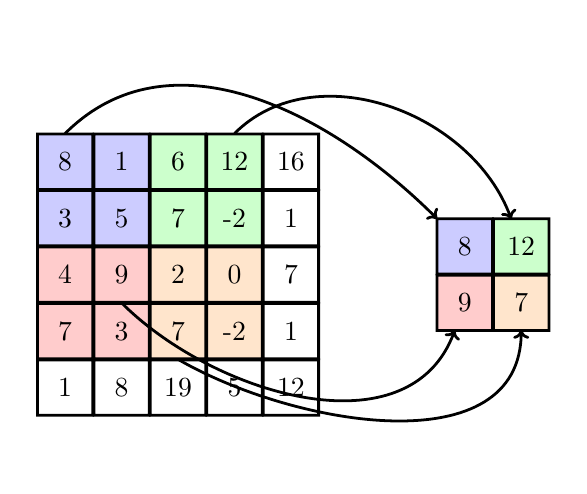
\begin{tikzpicture}
  % The matrix of nodes option here means every cell by default is a node
  \begin{scope}[transparency group]
    \begin{scope}[blend mode=multiply]
      \matrix (m) [matrix of nodes,nodes={draw,inner sep=0,minimum size=20},column
        sep=0, row sep =0] at (0,0) {%
         8 &  1 & 6 &  12 &  16 \\
         3 &  5 & 7 &  -2 &  1 \\
         4 &  9 & 2 &  0  &  7 \\
         7 &  3 & 7 &  -2 &  1 \\
         1 &  8 & 19 &  5  &  12 \\
      };
      \fill[blue!20] (m-1-1.north west) rectangle (m-2-2.south east);
      \fill[green!20] (m-1-3.north west) rectangle (m-2-4.south east);
      \fill[red!20] (m-3-1.north west) rectangle (m-4-2.south east);
      \fill[orange!20] (m-3-3.north west) rectangle (m-4-4.south east);

      \matrix (m2) [matrix of nodes,nodes={draw,inner sep=0, minimum size =20}, 
                    column sep=0,row sep=0] at (4,0) {%
        |[fill=blue!20]| 8 & |[fill=green!20]| 12 \\
        |[fill=red!20]|  9 & |[fill=orange!20]| 7 \\
      };
      \draw [->] (m-1-1.north) to [out=45,in=135] (m2-1-1);
      \draw [->] (m-1-4.north) to [out=45,in=110] (m2-1-2);
      \draw [->] (m-3-2.south) to [out=315,in=250] (m2-2-1);
      \draw [->] (m-4-3.south) to [out=330,in=270] (m2-2-2);
    \end{scope}
  \end{scope}
\end{tikzpicture}

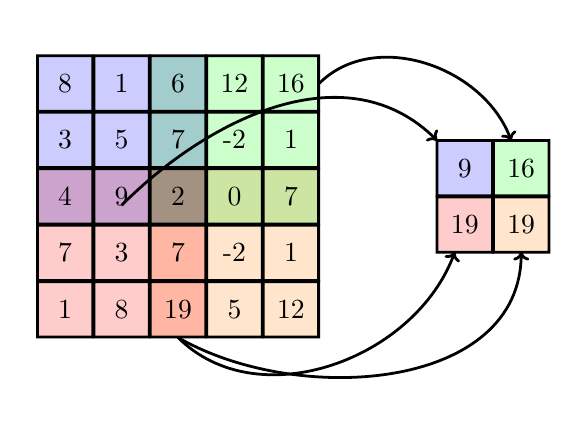
\begin{tikzpicture}
  % The matrix of nodes option here means every cell by default is a node
  \begin{scope}[transparency group]
    \begin{scope}[blend mode=multiply]
      \matrix (m) [matrix of nodes,nodes={draw,inner sep=0,minimum size=20},column
        sep=0, row sep =0] at (0,0) {%
         8 &  1 & 6 &  12 &  16 \\
         3 &  5 & 7 &  -2 &  1 \\
         4 &  9 & 2 &  0  &  7 \\
         7 &  3 & 7 &  -2 &  1 \\
         1 &  8 & 19 &  5  &  12 \\
      };
      \fill[blue!20] (m-1-1.north west) rectangle (m-3-3.south east);
      \fill[green!20] (m-1-3.north west) rectangle (m-3-5.south east);
      \fill[red!20] (m-3-1.north west) rectangle (m-5-3.south east);
      \fill[orange!20] (m-3-3.north west) rectangle (m-5-5.south east);
      \matrix (m2) [matrix of nodes,nodes={draw,inner sep=0, minimum size =20}, 
                    column sep=0,row sep=0] at (4,0) {%
        |[fill=blue!20]| 9 & |[fill=green!20]| 16 \\
        |[fill=red!20]| 19 & |[fill=orange!20]| 19 \\
      };
      \draw [->] (m-3-2.base) to [out=45,in=135] (m2-1-1);
      \draw [->] (m-1-5.east) to [out=45,in=110] (m2-1-2);
      \draw [->] (m-5-3.south) to [out=315,in=250] (m2-2-1);
      \draw [->] (m-5-3.south) to [out=330,in=270] (m2-2-2);
    \end{scope}
  \end{scope}
\end{tikzpicture}

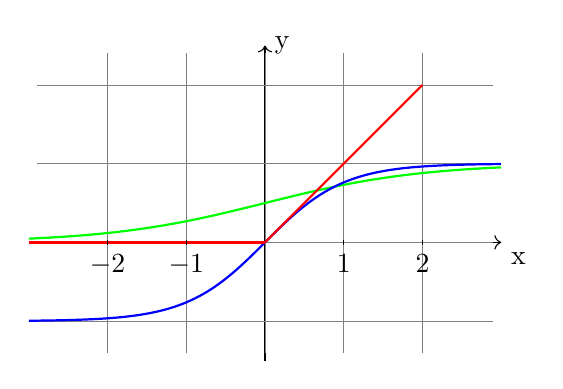
\begin{tikzpicture}
\draw[->] (-3,0) -- (3,0) node[below right] {x};
\draw[->] (0,-1.5) -- (0,2.5) node[right] {y};
\draw[step=1cm,gray,very thin] (-2.9,-1.4) grid (2.9, 2.4);
\draw[green, thick, domain=-3:3, samples=200] plot (\x, {1/(1+exp(-\x))});
\draw[blue, thick, domain=-3:3, samples=200] plot (\x, {(exp(\x)-exp(-\x))/(exp(\x)+exp(-\x))});
\draw[red, thick, domain=-3:0, samples=5] plot (\x, {0});
  \draw[red, thick, domain=0:2, samples=5] plot (\x, {\x});

\foreach \x in {-2,-1,1,2}
  \draw (\x cm,1pt) -- (\x cm,-1pt) node[anchor=north] {$\x$};
\end{tikzpicture}


\begin{tikzpicture}
  \tikzset{arrowstyle/.style={draw=gray!20, single arrow,minimum
    height=#1, single arrow, single arrow head extend=.4cm,}}

  \newcommand{\tikzfancyarrow}[2][2cm]{\tikz[baseline=-0.5ex]\node[arrowstyle=#1] {#2};}

  \tikzfancyarrow{}
  \draw[line width = 10pt, color=gray!20, arrows = {-Latex
\end{tikzpicture}

\end{document}
